\documentclass[12pt,a4paper]{article}
\usepackage[style = authoryear, maxcitenames = 1, uniquelist=false, sorting = nyt, abbreviate = true, doi = true, backend = biber]{biblatex}
\usepackage[lmargin = 3.5cm, rmargin = 3.5cm, tmargin = 2.5cm, bmargin = 2.5cm]{geometry}
\usepackage[onehalfspacing]{setspace}
\usepackage{graphicx}
\usepackage{hyperref}
\usepackage{times}
\usepackage{csquotes}
\usepackage[UKenglish]{babel}
\usepackage[textsize=tiny]{todonotes}
\usepackage[acronym]{glossaries}
\usepackage{soul} % for command \hl
\usepackage{pdfpages} % to insert pdf docs
\usepackage{csvsimple} % to import .csv files as tables
\usepackage{siunitx}
\usepackage{tikz}
\usepackage{caption} 
\usepackage{float}
\captionsetup[table]{skip=10pt} % more space between table and caption

\AtBeginBibliography{\small}
\addbibresource{main_sources.bib}

\setlength{\parindent}{0cm}
\setlength{\marginparwidth}{3.5cm} % make todonotes wider
\newcommand{\todoleft}[1]{{\reversemarginpar \todo{#1}}}


%%%%%%%%%%%%%%%%%%%%%%%%%%%%%%%%%%%%%%%%%%%%%%%%%%%%%%%%%%%%%%%%%%
\begin{document}
\def\findate{\today}


%title page
\thispagestyle{empty}
\begin{center}
    \Large{University of Innsbruck \\ Faculty of Mathematics, Computer Science and Physics} \\
    \vspace{3mm}
    \large{Institute for Theoretical Physics}
    \vspace{10mm}

    \includegraphics[width = 0.6 \linewidth]{logo.jpg}

    \vspace{10mm}
    \Large{Bachelor Thesis} \\
    \large{submitted for the degree of} \\
    \Large{Bachelor of Science} \\
    \vspace{10mm}
    \LARGE{\textbf{An information-theoretical approach to internal models in a Partially Observable Markov Decision Process}} \\
    \vspace{10mm}

    \large{by \\ Lukas Prader \\ Matriculation Nr.: 12115058 \\ SE Seminar with Bachelor Thesis}
\end{center}

\vspace{30mm}
\begin{tabular}{ll}
    \large{Submission Date:} & \large{\findate}                          \\
    \large{Supervisors:}     & \large{Alexander Vining, Hans J  Briegel} \\
\end{tabular}


\newpage
\thispagestyle{empty}
\begin{abstract}
    Lorem ipsum
\end{abstract}

\pagenumbering{roman}

\newpage
\tableofcontents
\thispagestyle{empty}
\newpage
\pagenumbering{arabic}

\section{Introduction} \label{chap:introduction}

\section{Results} \label{chap:results}

\subsection{Markov Process Plots}

% delayed action mdp
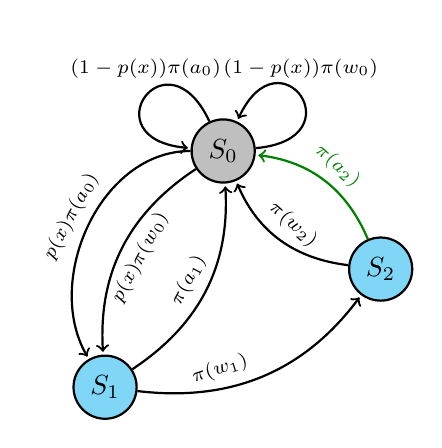
\begin{tikzpicture}[->,shorten >=1pt,auto,node distance=3cm,
        thick,main node/.style={circle,draw,font=\sffamily\Large\bfseries}]

    \node[fill=gray!50, circle, draw=black] (0) at (0,0) {$S_0$};
    \node[fill=cyan!50, circle, draw=black] (1) at (-1.5,-3) {$S_1$};
    \node[fill=cyan!50, circle, draw=black] (2) at (2,-1.5) {$S_2$};

    \path[every node/.style={font=\sffamily\scriptsize}]
    (0) edge [in=175,out=115, loop] node[above=3pt] {$(1-p(x)) \pi(a_0)$} (0)
    (0) edge [in=65,out=5, loop] node[above=3pt] {$(1-p(x)) \pi(w_0)$} (0)
    (0) edge [in=120,out=180] node[above, rotate=62] {$p(x) \pi(a_0)$} (1)
    (0) edge [bend right] node[below, rotate=62] {$p(x) \pi(w_0)$} (1)
    (1) edge [bend right] node[above, rotate=62] {$\pi(a_1)$} (0)
    (1) edge [bend right] node[rotate=18] {$\pi(w_1)$} (2)
    (2) edge [bend left] node[above, rotate=-42] {$\pi(w_2)$} (0)
    (2) edge [bend right, black!50!green] node[above, rotate=-42] {$\pi(a_2)$} (0);

\end{tikzpicture}

% delayed action with light observation
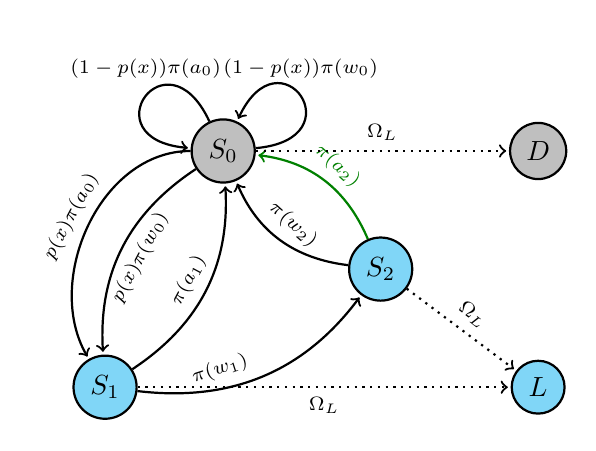
\begin{tikzpicture}[->,shorten >=1pt,auto,node distance=3cm,
        thick,main node/.style={circle,draw,font=\sffamily\Large\bfseries}]

    \node[fill=gray!50, circle, draw=black] (0) at (0,0) {$S_0$};
    \node[fill=cyan!50, circle, draw=black] (1) at (-1.5,-3) {$S_1$};
    \node[fill=cyan!50, circle, draw=black] (2) at (2,-1.5) {$S_2$};
    \node[fill=gray!50, circle, draw=black] (D) at (4,0) {$D$};
    \node[fill=cyan!50, circle, draw=black] (L) at (4,-3) {$L$};

    \path[every node/.style={font=\sffamily\scriptsize}]
    (0) edge [in=175,out=115, loop] node[above=3pt] {$(1-p(x)) \pi(a_0)$} (0)
    (0) edge [in=65,out=5, loop] node[above=3pt] {$(1-p(x)) \pi(w_0)$} (0)
    (0) edge [in=120,out=180] node[above, rotate=62] {$p(x) \pi(a_0)$} (1)
    (0) edge [bend right] node[below, rotate=62] {$p(x) \pi(w_0)$} (1)
    (1) edge [bend right] node[above, rotate=62] {$\pi(a_1)$} (0)
    (1) edge [bend right] node[rotate=18] {$\pi(w_1)$} (2)
    (2) edge [bend left] node[above, rotate=-42] {$\pi(w_2)$} (0)
    (2) edge [bend right, black!50!green] node[above, rotate=-42] {$\pi(a_2)$} (0)
    (0) edge [dotted] node[above] {$\Omega_L$} (D)
    (1) edge [dotted] node[below] {$\Omega_L$} (L)
    (2) edge [dotted] node[above, rotate=-38] {$\Omega_L$} (L);

\end{tikzpicture}

% reduced light model
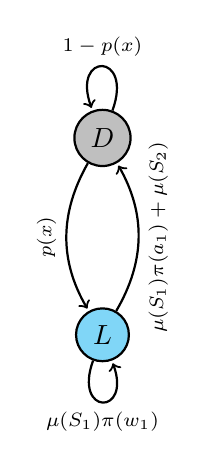
\begin{tikzpicture}[->,shorten >=1pt,auto,node distance=3cm,
        thick,main node/.style={circle,draw,font=\sffamily\Large\bfseries}]

    \node[fill=gray!50, circle, draw=black] (D) at (4,0) {$D$};
    \node[fill=cyan!50, circle, draw=black] (L) at (4,-2.5) {$L$};

    \path[every node/.style={font=\sffamily\scriptsize}]
    (D) edge [in=110,out=70, loop] node[above] {$1-p(x)$} (D)
    (D) edge [bend right] node[above, rotate=90] {$p(x)$} (L)
    (L) edge [bend right] node[below, rotate=90] {$\mu(S_1)\pi(a_1) + \mu(S_2)$} (D)
    (L) edge [in=290,out=250, loop] node[below] {$\mu(S_1)\pi(w_1)$} (L);

\end{tikzpicture}

% reduced action model
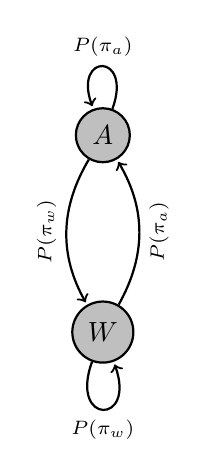
\begin{tikzpicture}[->,shorten >=1pt,auto,node distance=3cm,
        thick,main node/.style={circle,draw,font=\sffamily\Large\bfseries}]

    \node[fill=gray!50, circle, draw=black] (A) at (4,0) {$A$};
    \node[fill=gray!50, circle, draw=black] (W) at (4,-2.5) {$W$};

    \path[every node/.style={font=\sffamily\scriptsize}]
    (A) edge [in=110,out=70, loop] node[above] {$P(\pi_a)$} (A)
    (A) edge [bend right] node[above, rotate=90] {$P(\pi_w)$} (W)
    (W) edge [bend right] node[below, rotate=90] {$P(\pi_a)$} (A)
    (W) edge [in=290,out=250, loop] node[below] {$P(\pi_w)$} (W);

\end{tikzpicture}

% heads tails biased coin
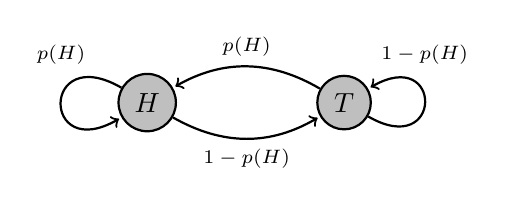
\begin{tikzpicture}[->,shorten >=1pt,auto,node distance=3cm,
        thick,main node/.style={circle,draw,font=\sffamily\Large\bfseries}]

    \node[fill=gray!50, circle, draw=black] (H) at (0,0) {$H$};
    \node[fill=gray!50, circle, draw=black] (T) at (2.5,0) {$T$};

    \path[every node/.style={font=\sffamily\scriptsize}]
    (H) edge [in=210,out=150, loop] node[above=10pt] {$p(H)$} (H)
    (H) edge [bend right] node[below] {$1-p(H)$} (T)
    (T) edge [bend right] node[above] {$p(H)$} (H)
    (T) edge [in=30,out=330, loop] node[above=10pt] {$1-p(H)$} (T);

\end{tikzpicture}

% skinner video process
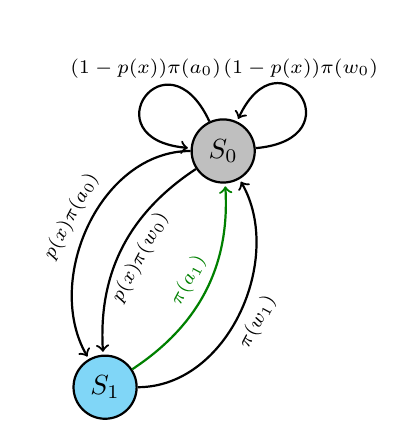
\begin{tikzpicture}[->,shorten >=1pt,auto,node distance=3cm,
        thick,main node/.style={circle,draw,font=\sffamily\Large\bfseries}]

    \node[fill=gray!50, circle, draw=black] (0) at (0,0) {$S_0$};
    \node[fill=cyan!50, circle, draw=black] (1) at (-1.5,-3) {$S_1$};

    \path[every node/.style={font=\sffamily\scriptsize}]
    (0) edge [in=175,out=115, loop] node[above=3pt] {$(1-p(x)) \pi(a_0)$} (0)
    (0) edge [in=65,out=5, loop] node[above=3pt] {$(1-p(x)) \pi(w_0)$} (0)
    (0) edge [in=120,out=180] node[above, rotate=62] {$p(x) \pi(a_0)$} (1)
    (0) edge [bend right] node[below, rotate=62] {$p(x) \pi(w_0)$} (1)
    (1) edge [bend right, black!50!green] node[above, rotate=62] {$\pi(a_1)$} (0)
    (1) edge [in=300,out=0] node[below, rotate=62] {$\pi(w_1)$} (0);

\end{tikzpicture}

% L=2 light process
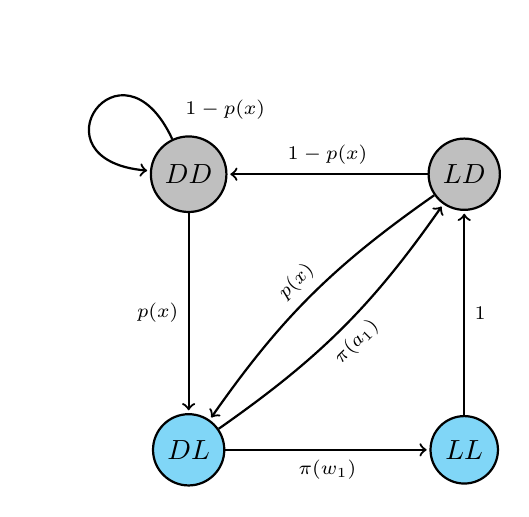
\begin{tikzpicture}[->,shorten >=1pt,auto,node distance=3cm,
    thick,main node/.style={circle,draw,font=\sffamily\Large\bfseries}]

\node[fill=gray!50, circle, draw=black] (DD) at (0,3.5) {$DD$};
\node[fill=gray!50, circle, draw=black] (LD) at (3.5,3.5) {$LD$};
\node[fill=cyan!50, circle, draw=black] (DL) at (0,0) {$DL$};
\node[fill=cyan!50, circle, draw=black] (LL) at (3.5,0) {$LL$};

\path[every node/.style={font=\sffamily\scriptsize}]
(DD) edge [in=175,out=115, loop] node[right=1cm] {$1-p(x)$} (DD)
(DD) edge node[left] {$p(x)$} (DL)
(DL) edge [bend right=10]  node[below, rotate=45] {$\pi(a_1)$} (LD)
(LD) edge [bend right=10]  node[above, rotate=45] {$p(x)$} (DL)
(LD) edge node[above] {$1-p(x)$} (DD)
(DL) edge node[below] {$\pi(w_1)$} (LL)
(LL) edge node[right] {$1$} (LD);

\end{tikzpicture}

\section{Conclusion} \label{chap:conclusion}


\section{Acknowledgements} \label{chap:acknowledgements}


\clearpage
\section*{Declaration of Authorship}

I hereby solemnly declare, by my own signature, that I have independently authored the presented work and have not used any sources or aids other than those indicated. All passages taken verbatim or in content from the specified sources are identified as such.

I consent to the archiving of this Bachelor thesis.

\hfill
\vspace{2cm} Innsbruck, \findate \hfill Lukas Prader \includegraphics[height = 10mm]{"signature.png"}


\newpage
\printbibliography[]
\input{appendix}

\end{document}